\documentclass[9pt,conference]{IEEEtran}
\usepackage[utf8]{inputenc}
\usepackage[brazil]{babel}

% Diversos
\usepackage{csquotes}
\usepackage{graphicx}
\usepackage{verbatim}
\usepackage{hyperref}
\usepackage{smartdiagram}

% Título
\title{Utilizando Redes Convolucionais de Grafos Espaço-Temporais para o Reconhecimento da Línguas de Sinais}
%\author{Cleison Correia de Amorim}
\date{Outubro 2018}

\author{
    \IEEEauthorblockN{Cleison Correia de Amorim}
    \IEEEauthorblockA{Centro de Informática\\
    Universidade Federal de Pernambuco\\
    Email: cca5@cin.ufpe.br}
}

% Comandos
% 'image': definição de imagem
\newcommand{\image}[4][\linewidth] {
    \begin{figure}[ht]
    \centering
    \includegraphics[width=#1]{#3}
    \caption{#4}
    \label{#2}
    \end{figure}
}

% 'refimage': referências de imagens
\newcommand{\refimage}[1] {figura \ref{#1}}

% 'refsection': referências de seções
\newcommand{\refsect}[1] {seção "\nameref{#1}"}


\begin{document}
\maketitle
\begin{abstract}
O reconhecimento de sinais é uma área de pesquisa com diversos desafios, mas que possui um papel importante de facilitar a comunicação do Surdo e de remover as barreiras ainda existentes nessa comunicação para com a sociedade. Este trabalho propõe a utilização de um modelo de aprendizagem profunda de identificação de ações conhecido como Rede Convolucional de Grafos Espaço-Temporais para promover o reconhecimento da língua de sinais. Trata-se de uma nova abordagem centrada no movimento do esqueleto humano que utiliza grafos para capturar seu movimento sob duas dimensões, espacial e temporal, e que é capaz de considerar aspectos complexos da dinâmica dessa língua. Além disso, este trabalho também apresenta a criação de um \textit{dataset} de esqueletos humanos para a língua de sinais baseado no ASLLVD, o qual é utilizado neste estudo e disponibilizado publicamente com o intuito de contribuir para o desenvolvimento de estudos futuros relacionados.
\end{abstract}

\begin{IEEEkeywords}
Língua de Sinais, Redes Neurais Convolucionais, Grafos Espaço-Temporais.
\end{IEEEkeywords}


\section{Introdução} %%%%%%%%%%%%%%%%%%%%%%%%%%%%%%%%%%%%%%%%%%%
\label{sec:introducao}

A língua de sinais é uma ferramenta de comunicação visual que possibilita com que indivíduos com diferentes tipos de deficiência auditiva comuniquem-se entre si e com os demais indivíduos na sociedade. É a língua utilizada pela maioria dos Surdos em seu cotidiano e, muito além disso, é o símbolo de identificação entre os membros dessa comunidade e a principal força que os une. 
Ela possui uma relação muito estreita com a cultura dos países onde é utilizada e, por esse motivo, cada uma dessas nações possui uma língua própria nascida e desenvolvida com as suas comunidades Surdas \cite{pereira-choi-2011}.

Segundo a Organização Mundial de Saúde, o número de pessoas surdas é de cerca de 466 milhões e estima-se que até 2050 esse número ultrapasse os 900 milhões -- o que equivale a uma previsão de 1 em cada 10 indivíduos ao redor do mundo \cite{who-2018}. Esses dados, por sua vez, ressaltam a abrangência e a importância da língua sinalizada na comunicação dessas pessoas em diferentes nações. 

Apesar disso, hoje ainda é pequeno o número de pessoas ouvintes que são capazes de se comunicar por meio dessa língua. Isso acaba caracterizando uma barreira invisível que interfere na comunicação entre as comunidades Surdos e ouvintes, inviabilizando uma integração mais efetiva entre essas pessoas \cite{peres-2006}. Nesse contexto, faz-se extremamente importante desenvolver ferramentas que sejam capazes de preencher essa lacuna promovendo a integração entre essas pessoas. 

Por essa razão, estudos relacionados com o reconhecimento da língua de sinais vêm sendo desenvolvidos desde a década de 1990 e é possível constatar resultados significativos a partir deles \cite{lim-2016, recent-advances-dl-2017}. Os principais desafios encontrados por eles estão relacionados primeiramente com a necessidade de considerar os aspectos dinâmicos dessa língua, como os movimentos, articulações entre partes do corpo e as expressões não-manuais, ao invés de apenas se limitarem a reconhecer sinais estáticos ou posições de mãos isoladas. Além disso, ela apresenta milhares de sinais, que às vezes diferem-se apenas por mudanças sutis no movimento, forma ou posição da mão e envolvem sobreposições significativas de dedos e oclusões. Quando combinadas às diferenças no estilo de sinalização por indivíduos distintos e às variações decorrentes da não-universalidade e regionalismos, essa linha de pesquisa pode tornar-se desafiadora o suficiente para os atuais algoritmos de inteligência computacional \cite{konstantinidis-2018}.

Este trabalho, portanto, apresenta a aplicação nessa área de pesquisa de uma nova abordagem capaz de realizar o reconhecimento de ações humanas tomando como base grafos espaço-temporais, a qual é denominada Redes Convolucionais de Grafos Espaço Temporais (ou \textit{Spatial-Temporal Graph Convolutional Networks} - ST-GCN) \cite{st-gcn-2018}.
Ao utilizar representações em grafos do esqueleto humano, essa técnica centraliza o foco no movimento do corpo e nas interações entre suas partes, desconsiderando a interferência do ambiente à sua volta. Além disso, ela também aborda os movimentos dos indivíduos sob as dimensões espacial e temporal, e isso lhe permite capturar os aspectos dinâmicos das ações exercidas no decorrer do tempo. Essas características fazem dessa uma abordagem relevante para lidar com os desafios e particularidades do reconhecimento da língua sinalizada.

Entretanto, para que fosse possível aplicar o método acima, foi necessário primeiro desenvolver um \textit{dataset} de esqueletos humanos da língua de sinais que viria a servir como a informação principal para alimentar o ST-GCN e possibilitar a criação de seus grafos espaço-temporais. Para isso, utilizou-se como base o \textit{American Sign Language Lexicon Video Dataset} (ASLLVD), que consiste num amplo conjunto de sinais da língua americana, a partir dos quais foram segmentados, estimados e extraídos os esqueletos necessários a técnica apresentada.

Sendo assim, este trabalho traz como principais contribuições: 1) a adoção no reconhecimento de sinais de uma nova técnica centrada no movimento humano, que considera diferentes aspectos da dinâmica dessa língua e que contribui para superar alguns dos principais desafios apontados acima; 2) a criação de um novo \textit{dataset} de esqueletos humanos para a língua de sinais, o qual objetiva suportar trabalhos futuros e apoiar o desenvolvimento de estudos nessa área.

Este trabalho está organizado da seguinte forma: na seção \ref{sec:trabalhos-relacionados} são apresentados os trabalhos relacionados e o funcionamento do ST-GCN em maiores detalhes; a seção \ref{sec:experimentos} aborda a condução dos experimentos, incluindo o processo de criação do novo \textit{dataset} e os ajustes realizados no ST-GCN para o reconhecimento de sinais; por fim, na seção seção \ref{sec:resultados} estão contidos os resultados obtidos a partir da abordagem aplicada.



\section{Trabalhos Relacionados} %%%%%%%%%%%%%%%%%%%%%%%%%%%%%%%%%%%%%%%%%%%%%%%%%%%%%%%%%%%%%%%%%%%%
\label{sec:trabalhos-relacionados}

O reconhecimento de línguas de sinais tem apresentado progressos relevantes nos últimos anos, os quais são motivados principalmente pelo advento de sensores modernos, de novas técnicas de aprendizagem de máquina e de \textit{hardwares} mais potentes que viabilizam o surgimento de algoritmos mais robustos \cite{recent-advances-dl-2017, recent-advances-sl-2013}. Além disso, abordagens consideradas intrusivas e que requeriam o uso de sensores como luvas, acelerômetros e marcadores acoplados ao corpo do interlocutor vêm sendo aos poucos abandonadas, cedendo espaço para novas abordagens utilizando câmeras convencionais e técnicas de visão computacional. 

Devido a esse movimento, é perceptível também o aumento na adoção de técnicas de extração de características como SIFT \cite{lowe-2004}, HOG \cite{dalal-2005}, HOF \cite{laptev-2008} e STIP \cite{laptev-2008} \cite{recent-advances-dl-2017} afim de pré-processar as imagens obtidas por essas câmeras e fornecer informações mais ricas para uso pelos algoritmos de aprendizagem \cite{lim-2016, shanta-2018}.

%Nessa linha, em \cite{lim-2016} foi introduzida uma abordagem derivada do HOF que é denominada de Histograma de Fluxo Óptico Baseado em Blocos de representação (ou \textit{Block-Based Histogram of Optical Flow} - BHOF) para o reconhecimento da linguagem de sinais a partir das imagens das mãos. Nele, primeiramente a face do signatário é rastreada e removida, e o modelo de segundo plano é construído por meio da fusão dos filtros mediano e de moda em toda a sequência de vídeo para detectar as mãos. Com base nesse modelo de segundo plano, o primeiro plano é então extraído e a posição da mão é determinada. Em seguida, as regiões do fluxo óptico das mãos são extraídas e o fluxo óptico do histograma baseado em blocos é finalmente calculado e utilizado na classificação. 

As Redes Neurais Convolucionais (ou CNNs) têm se sobressaído nos últimos anos como o algoritmo com presença mais expressiva na resolução de problemas de reconhecimento de sinais. Seus resultados são notáveis e comumente sua acurácia é capaz de superar 90\%  \cite{shanta-2018, ji-2017, taskiran-2018, rao-2018}. Algumas de suas variações encontradas, são as 3D CNNs \cite{elbadawy-2017}, a combinação com outros modelos como o Inception \cite{das-2018} ou ainda a aplicação de Regiões de Interesse \cite{sajanraj-2018}. Em menor proporção, também é constatada a adoção de Redes Neurais Recorrentes \cite{konstantinidis-2018} e de Redes Residuais Temporais \cite{pigou-2017} com esse mesmo objetivo.

Apesar dos avanços acima, uma grande parcela desses estudos ainda se restringe a abordar o problema dos sinais por meio de imagens estáticas ou de letras isoladas da datilologia\footnote{
     Datilologia – também conhecida como alfabeto digital ou alfabeto manual. Consiste na soletração de palavras pelos Surdos. É geralmente utilizada para introduzir uma palavra que ainda não possui um sinal equivalente \cite{quadros-2004, pereira-choi-2011}.
} \cite{shanta-2018, taskiran-2018, elbadawy-2017, das-2018, sajanraj-2018}. Isso é ruim porque faz com que seja desconsidera a dinâmica intrínseco à língua, como seus movimentos, expressões não-manuais e as articulações entre partes do corpo \cite{quadros-2004}. Nesse sentido, é extremamente relevante que novos estudos sejam capazes de observar características como essas, que são tão importantes para a língua, como em \cite{konstantinidis-2018} e \cite{pigou-2017}. 

Com esse propósito, o presente trabalho apresenta a utilização de uma abordagem de identificação de ações centrada no movimento do esqueleto humano para realizar o reconhecimento da língua de sinais. Essa técnica é conhecida como Rede Convolucional de Grafos Espaço-Temporais\footnote{
    Disponível em \url{https://github.com/yysijie/st-gcn}.
} (ou \textit{Spatial-Temporal Graph Convolutional Network - ST-GCN}) e é introduzida em \cite{st-gcn-2018}. 

A motivação dessa técnica surgiu a partir da necessidade de métodos que fossem capazes de capturar de forma autônoma os padrões contidos na configuração espacial das articulações do corpo, bem como sua dinâmica temporal. Segundo seus autores, métodos anteriores de reconhecimento de ações através de esqueletos eram limitados por não explorarem explicitamente tais relações espaciais entre as articulações, que são cruciais para a compreensão das ações humanas. Esses métodos simplesmente empregavam as coordenadas conjuntas em etapas de tempo individuais para formar vetores de característica, aplicando uma análise temporal neles \cite{st-gcn-2018, wang-2012, fernando-2015}.

%Mais recentemente, eles afirmam, novos métodos que tentaram alavancar as conexões naturais entre as articulações foram desenvolvidos \cite{shahroudy-2016, yong-du-2015}. Eles mostraram melhorias encorajadoras, o que sugere a importância da conectividade. No entanto, a maioria desses métodos baseia-se em partes ou regras criadas manualmente para analisar os padrões espaciais. Como resultado, os modelos criados para uma aplicação específica são difíceis de serem generalizados para outras \cite{st-gcn-2018}.

O ST-GCN tem como base de sua formulação uma sequência de grafos de esqueletos que representam o corpo humano, os quais são obtidos a partir de uma série de \textit{frames} de vídeos de ações de indivíduos. A figura \ref{fig:st-gcn-graph} permite-nos visualizar essa estrutura, onde cada nó corresponde a um ponto de articulação. Os vértices intra-corporais são definidos com base nas conexões naturais do corpo. Os vértices inter-frames, por sua vez, conectam as mesmas articulações entre \textit{frames} consecutivos para denotar sua trajetória no decorrer do tempo \cite{st-gcn-2018}.

\image
	[3.5cm]
    {fig:st-gcn-graph}
    {images/st_gcn_graph}
    {Sequência de grafos de esqueletos, que denotam o movimento humano no espaço e no tempo, utilizados pelo ST-GCN. Fonte: \cite[p. 1]{st-gcn-2018}.}

A figura \ref{fig:st-gcn-workflow} apresenta uma visão geral da abordagem utilizada por essa técnica. Nela, primeiro é realizada a estimação dos esqueletos dos indivíduos nos vídeos de entrada e a construção de grafos espaço-temporais com base neles. Em seguida, múltiplas camadas de convolução ST-GCN são aplicadas gerando, gradualmente, mapas de características de nível cada vez mais alto para os grafos apresentados. Por fim, eles são submetidos a um classificador para a identificação da ação correspondente.

\image
    {fig:st-gcn-workflow}
    {images/st_gcn_workflow}
    {Fluxo do ST-GCN, onde os grafos criados a partir dos indivíduos presentes nos vídeos são submetidos ao modelo e, por fim, classificados entre as ações disponíveis. Fonte: \cite[p. 3]{st-gcn-2018}.}


% Funcionamento do ST-GCN:

Para compreender o funcionamento do ST-GCN em mais detalhes, é preciso primeiro introduzir as estratégias de amostragem e de particionamento adotadas por ele. Quando lidamos com convoluções sobre imagens 2D, é fácil imaginar a existência de um \textit{grid} rígido (ou retângulo) em volta de um ponto central que representa a área de amostragem do filtro convolucional e delimita sua vizinhança. No caso dos grafos, entretanto, é necessário ir além dessa definição e passar a considerar que a vizinhança do ponto central será composta pelos pontos que estão diretamente conectados a ele por um vértice. A figura \ref{fig:st-gcn-sampling} permite visualizar essa definição para um único \textit{frame}. Observe que para os pontos centrais em vermelho, agora as bordas tracejadas passam a representar a área de amostragem do filtro convolucional. Observe também que apesar de haver outros pontos fisicamente próximos aos pontos centrais (como no exemplo dos pontos dos pés, joelhos e cintura), a menos que haja um vértice que os conecte.

\image
	[2.5cm]
    {fig:st-gcn-sampling}
    {images/st_gcn_sampling}
    {Representação da convolução em um grafo. As articulações do corpo são desenhadas com pontos azuis. Os pontos vermelhos representam os pontos centrais de um filtro com distância D = 1 aplicado ao \textit{frame}, cuja abrangência é delimitada pela linha tracejada. Fonte: \cite[p. 5]{st-gcn-2018}.}

Por meio da figura \ref{fig:st-gcn-sampling} é possível observar que apenas estão sendo considerados pelo filtro convolucional os pontos que estão imediatamente conectados aos pontos centrais. Em outras palavras, diz-se que a área de \textbf{amostragem} desse filtro está delimitada para vizinhos com distância D = 1. Essa distância é a mesma considerada pelos autores no ST-GCN \cite{st-gcn-2018}.

\image
	[2.5cm]
    {fig:st-gcn-spatial-part}
    {images/st_gcn_spatial_partitioning}
    {No Particionamento de Configuração Espacial, os nós são rotulados de acordo com suas distâncias ao centro de gravidade do esqueleto (cruz preta) comparado com o do nó raiz (verde). Os nós centrípetos têm distâncias menores (azul), enquanto os nós centrífugos têm distâncias mais longas (amarelo) do que o nó raiz. Fonte: \cite[p. 5]{st-gcn-2018}.}
    
A estratégia de \textbf{particionamento}, por sua vez,  está baseada na localização das articulações e nas características do movimento do corpo humano, conforme ilustra a figura \ref{fig:st-gcn-spatial-part}. De acordo com os autores, ela motiva-se no fato de que os movimentos das partes do corpo poderem ser categorizados como concêntricos ou excêntricos e, por isso, os pontos na região de amostragem são particionados em três subconjuntos:

\begin{enumerate}
    \item O nó raiz (ou ponto central, sinalizado em verde na imagem);
    \item O grupo centripetal (pontos em azul na imagem), que são os nós da vizinhança que estão mais próximos do centro de gravidade do esqueleto (cruz preta na imagem) do que o nó raiz;
    \item O grupo centrifugal (pontos em amarelo na imagem), que são os nós mais distante do centro de gravidade do que o nó raiz;
\end{enumerate}

O centro de gravidade é definido como sendo a coordenada média de todas as juntas do esqueleto em um \textit{frame}. Durante a convolução, cada ponto do corpo é rotulado segundo uma das partições acima. A essa estratégia os autores atribuem o nome de Particionamento de Configuração Espacial. É através desse método que os autores também estabelecem os pesos do modelo, fazendo com que cada uma das partições receba um peso distinto a ser aprendido.

%Uma vez exploradas as estratégias definidas pelo ST-GCN, apresentadas sob o contexto de um único \textit{frame} na dimensão espacial, é possível aprofudar essa discussão para compreender como o modelo considera a dimensão temporal. 

Para aprender a dimensão temporal, o ST-GCN estende o conceito de convolução de grafos acima para o esquema apresentado na figura \ref{fig:st-gcn-convolution}. Consideremos o apresentado na figura \ref{fig:st-gcn-graph}, que define que essa dimensão é representada pela sequência de grafos de esqueletos de \textit{frames} empilhados de forma consecutiva. Com isso, temos em mãos um conjunto de grafos em sequência que são vizinhos entre si. Consideremos agora que cada articulação do corpo existente em um grafo possui um vértice que conecta-se a ela mesma no grafo vizinho do \textit{frame} anterior e também do \textit{frame} posterior. Dado isso, se retomarmos à definição de amostragem perceberemos que o filtro convolucional passará agora a contemplar também esses pontos nos grafos vizinhos, uma vez que eles passam a se enquadrar nos requisitos de estarem diretamente conectados e a uma distância D = 1. É, portanto, dessa forma que o ST-GCN é capaz de considera as dimensões espacial e temporal e aplicar convoluções sobre elas.

\image
	[7cm]
    {fig:st-gcn-convolution}
    {images/st_gcn_convolution}
    {Convolução sob as dimensões espacial e temporal, que considera os pontos diretamente conectados no grafo atual e nos grafos vizinhos. Fonte: \cite[p. 3]{st-gcn-2018}.}


% Arquitetura:

A figura \ref{fig:st-gcn-architecture} (à esquerda) permite-nos visualizar a arquitetura do modelo e suas camadas de convolução. Ao todo, são nove camadas convolucionais ST-GCN posicionadas de forma sequencial, que realizam a extração das características dos grafos espaço-temporais. Elas são precedidas por uma camada de normalização e seguidas por uma camada de \textit{pooling} global e outra de classificação \textit{softmax}. À direita da imagem é apresentado também o detalhe de uma de suas unidades convolucionais.

\begin{figure}[ht]
    \centering
    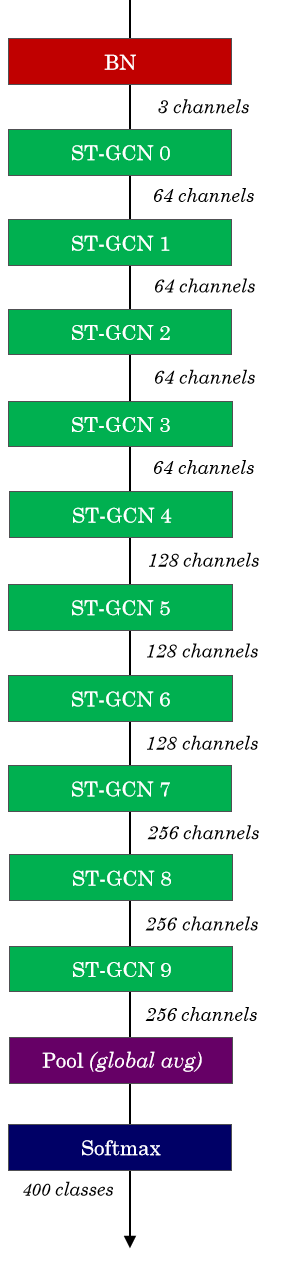
\includegraphics[width=2.5cm]{images/st_gcn_architecture}
    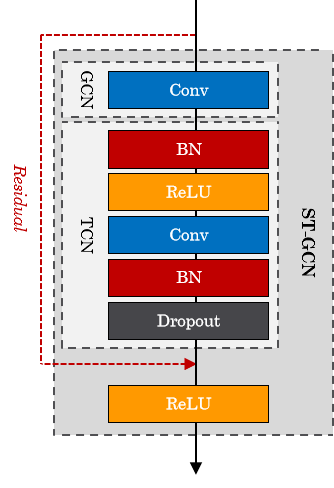
\includegraphics[width=3.0cm]{images/st_gcn_architeture_unit}
    \caption{Arquitetura do modelo (à esquerda) e detalhe de uma unidade ST-GCN (à direita). Unidades de ST-GCN aplicam operações de normalização, convolução, ativação e \textit{dropout} aos grafos e levam em consideração o valor residual da camada anterior para calcular as ativações de saída. Fonte: adaptado de \cite{st-gcn-2018}.}
    \label{fig:st-gcn-architecture}
\end{figure}


Para realizar a extração dos esqueletos a partir das ações dos indivíduos em \cite{st-gcn-2018}, os autores utilizaram uma biblioteca denominada OpenPose\footnote{
    Disponível em \url{https://github.com/CMU-Perceptual-Computing-Lab/openpose}.
}. Trata-se de uma ferramenta de código aberto que utiliza algoritmos de aprendizagem profunda para detectar e estimar até 135 pontos dos esqueletos de indivíduos em vídeos \cite{cao-realtime-2017, simon-hand-2017, wei-cpm-2016}. Apesar disso, os autores utilizaram apenas 18 desses pontos, os quais se correspondem às articulações principais do corpo (vide figura \ref{fig:keypoints-pose}). 

\image
	[3cm]
    {fig:keypoints-pose}
    {images/keypoints_pose_COCO_18}
    {Representação dos 18 pontos referentes ao corpo humano, extraídos pelo OpenPose. Fonte: \cite{openpose-output-2018}.}

% Todo o fluxo descrito até aqui trata da aplicação do ST-GCN para o contexto onde vídeos isolados são gravados previamente e utilizados como entrada. Apesar disso, entende-se que seria possível, com algum trabalho adicional, evoluí-lo na direção de substituir essa entrada por um \textit{streaming} de vídeo capturado em tempo real por uma câmera. Para isso, seria necessário passar a estimar continuamente com uma biblioteca ou \textit{hardware} específico as poses dos \textit{frames} capturados, provendo assim um \textit{streaming} de esqueletos para o modelo. A biblioteca OpenPose (que está descrita em detalhes mais adiante) é capaz de atender a essa necessidade, porém seus requisitos de \textit{hardware} robusto podem acabar por limitar sua adoção em alguns contextos na prática. A leitura dos dados pelo modelo também precisaria ser evoluída afim de que ao invés de considerar informações em arquivos físicos, sejam utilizadas aquelas fornecidas pelo \textit{streaming} de esqueletos. Como o ST-GCN hoje só trabalha com vídeos de tamanho fixo, essa entrada em fluxo contínuo apenas seria classificada por ele de janelas em janelas de tempo, quando completado em memória esse número fixo estabelecido de \textit{frames}.


\section{Experimentos} %%%%%%%%%%%%%%%%%%%%%%%%%%%%%%%%%%%%%%%%%%%%%%%%%%%%%%%%%%%%%%%%%%%%%%%
\label{sec:experimentos}

Esta seção define a abordagem utilizada para organizar e conduzir os experimentos deste trabalho. Em primeiro lugar, foi estabelecido como modelo o ST-GCN devido à capacidade de centrar sua atenção essencialmente no movimento corpo humano, desconsiderando a interferência do ambiente externo, conforme abordam as seções \ref{sec:introducao} e \ref{sec:trabalhos-relacionados}. Entende-se que esses aspectos são essenciais para que uma técnica aborde o reconhecimento da língua de sinais, que também possui como elemento principal o corpo humano e sua dinâmica.

Em seguida, foi estabelecido o \textit{dataset} a ser utilizado como referência, bem como as etapas de pré-processamento necessárias para criar uma novo conjunto compatível com o ST-GCN dentro dos objetivos deste trabalho. Por fim, foram realizados pequenos ajustes no modelo e conduzidos os treinamentos para coleta dos resultados deste trabalho.

%\begin{enumerate}
%    \item Definição do modelo: nesse passo foi selecionado o modelo ST-GCN e sua abordagem baseada em grafos para lidar com o problema da língua de sinais;
%    \item Definir \textit{dataset}: foi estabelecido o ASLLVD, devido à sua abrangência relevante de sinais, qualidade das amostras coletadas, organização das anotações e rotulações, e articulação dos sinais por indivíduos nativos. Apesar de baseado na Língua Americana de Sinais, a utilização desse \textit{dataset} não restringe a abordagem apresentada à língua daquele país. Ao contrário, entende-se que é possível adotar o mesmo método a \textit{datasets} de línguas de outros países;
%    \item Preparar \textit{dataset}: para que fosse possível utilizar o \textit{dataset} acima com o ST-GCN foi necessário primeiro criar um \textit{pipeline} de pré-processamento, conforme descrito mais adiante nesta seção, afim de colocar cada amostra em  um formato compatível com a entrada do modelo;
%    \item Adaptar modelo: para que fosse possível utilizar o ST-GCN no contexto da língua de sinais, foi necessário realizar pequenas adaptações na interpretação dos grafos e na leitura dos dados. Esse processo também está melhor descrito mais adiante;
%    \item Treinar modelo adaptado: nesse passo, o modelo acima será submetido às amostras do \textit{dataset} para que possa desenvolver um conhecimento acerca do problema;
%    \item Avaliar e melhorar resultados: a partir das descobertas obtidas na tarefa acima, serão realizados os eventuais ajustes no modelo, \textit{dataset} ou nas configurações do treinamento, e repetido o passo anterior.
%\end{enumerate}


\subsection{Dataset} %%%%%%%%%%%%%%%%%%%%%%%%%%%%%%%%%%%%%%%%%%%%%%%%%%%%%%%%%%%%%%%%%%%%%%%%%%%%%%%%%
\label{sec:dataset}

Foi selecionado para este trabalho o \textit{American Sign Language Lexicon Video Dataset} (ou ASLLVD). Ele consiste num \textit{dataset} público\footnote{
    Disponível em \url{http://csr.bu.edu/asl/asllvd/annotate/index.html}.
} amplo que contém sequências de vídeos de milhares de sinais distintos da Língua de Sinais Americana (\textit{American Sign Language}, ou ASL), bem como as anotações dessas sequências, os \textit{frames} de início e fim, e os rótulos de classe para cada sinal \cite{athitsos-asllvd-2008, neidle-2012, vloger-2012}.

Segundo os autores, cada sinal é articulado por indivíduos nativos da ASL, e as sequências de vídeo são coletadas utilizando um sistema de quatro câmeras que captura simultaneamente duas vistas frontais, uma vista lateral e uma vista ampliada da face desses indivíduos. A figura \ref{fig:asllvd-example} exemplifica a captura de três dessas vistas para o sinal "\textit{MERRY-GO-ROUND}".

\image
    {fig:asllvd-example}
    {images/asllvd_example}
    {Exemplo de captura do sinal \textit{"MERRY-GO-ROUND"} sob três perspectivas, no ASLLVD. Fonte:  \cite[p. 2]{athitsos-asllvd-2008}.}

Ainda de acordo com os autores, o número e o tipo de sinais incluídos no ASLLVD são semelhantes em escala e escopo ao conjunto de entradas lexicais nos dicionários existentes de "Inglês-para-ASL". Existe ao menos um exemplo de vídeo por sinal para quase todos os sinais contidos no Dicionário Gallaudet de Língua Americana de Sinais \cite{athitsos-asllvd-2008, gallaudet-2005}, os quais são articulados por indivíduos nativos. 

Ao analisar o \textit{dataset} em detalhe é possível identificar a existência de um total de 2.745 sinais, representados em aproximadamente 10 mil amostras. Cada sinal contém entre 1 e 18 amostras articuladas por diferentes indivíduos (sendo 4 o número médio de amostras por sinal).


\subsection{Criação do \textit{dataset} de esqueletos para a língua de sinais} %%%%%%%%%%%%%%%%%%%%%%%%%%%%%%%%%%%%%%%%%%%%%%%%%%%%%%%%%%%%%%%%%%%%%%%%%%%
\label{sec:criacao-dataset}

Para tornar as amostras do ASLLVD compatíveis com a entrada esperada pelo modelo ST-GCN foi necessário aplicar uma série de etapas de pré-processamento, as quais deram origem ao novo \textit{dataset} contendo a estimativa de esqueletos para todos os indivíduos e sinais contidos nele.

A esse novo \textit{dataset} foi atribuído o nome \textbf{ASLLVD-Skeleton}, e o mesmo foi disponibilizado publicamente\footnote{
    Disponível em \url{http://www.cin.ufpe.br/~cca5/asllvd-skeleton}
} com o intuito de contribuir com o desenvolvimento de estudos futuros no reconhecimento de línguas de sinais.

As etapas aplicadas na criação desse novo \textit{dataset} estão apresentadas na figura \ref{fig:preprocessamento} e descritas a seguir.

\image
    [8cm]
    {fig:preprocessamento}
    {pt/images/dataset_preprocessing}
    {Etapas de pré-processamento aplicadas na criação do \textit{dataset} ASLLVD-Skeleton.}

A primeira etapa consiste num passo preliminar de \textbf{obtenção dos vídeos} que compõem o ASLLVD de forma automática, afim de reconstitui-lo e viabilizar as etapas posteriores. Um arquivo de metadados\footnote{
    Disponível em \url{http://www.bu.edu/asllrp/dai-asllvd-BU_glossing_with_variations_HS_information-extended-urls-RU.xls}
} desse \textit{dataset} foi utilizado para guiar esse processo. Nesse momento foram considerados apenas os vídeos capturados pela câmera frontal, que contempla simultaneamente os movimentos do tronco, mãos e face dos indivíduos.

A etapa seguinte consiste em \textbf{segmentar os vídeos} para que seja obtido um vídeo por sinal. Isso se faz necessário porque cada arquivo no \textit{dataset} original corresponde a uma seção onde foram gravados múltiplos sinais por indivíduo. Com isso, é necessário constituir um novo conjunto organizado de tal forma que cada sinal esteja disposto individualmente com seu respectivo rótulo. Para isso, também foi considerado o arquivo de metadados comentado acima, que dispõe dos rótulos e das respectivas marcações de \textit{frames} de início e término para cada sinal nas seções. Como saída dessa etapa, tem-se pequenos vídeos com duração média de 1 a 5 segundos e com aspecto semelhante ao ilustrado na figura \ref{fig:sign-original}.

\image
    [4cm]
    {fig:sign-original}
    {images/sign_original}
    {Representação do sinal "EXAGGERATE", segmentado a partir das seções gravadas para o ASLLVD. Fonte: \cite{athitsos-asllvd-2008}.}

O terceiro passo consiste em realizar a \textbf{estimar os esqueletos} dos indivíduos presentes em cada vídeo segmentado. Em outras palavras, nesse momento são extraídas as coordenadas das articulações desses indivíduos, \textit{frame} a \textit{frame}, para compor os esqueletos que darão origem aos grafos utilizados pelo ST-GCN. Para isso, da mesma forma como em \cite{st-gcn-2018}, utilizou-se a biblioteca OpenPose. A diferença, no entanto, está no fato de que além das coordenadas referentes ao corpo, aqui foi adotado um número consideravelmente maior de coordenadas para abranger também as mãos e face dos indivíduos. No total são 130 pontos, dos quais 21 correspondem a cada uma das mãos; 70 correspondem às coordenadas da face; e 18 correspondem ao corpo (vide figura \ref{fig:keypoints-face-hand} e figura \ref{fig:keypoints-pose}). A figura \ref{fig:sign-pose}, por sua vez, ilustra a reconstrução em uma imagem 2D das coordenadas estimadas pelo OpenPose para o sinal "EXAGGERATE".


\begin{figure}[ht]
    \centering
    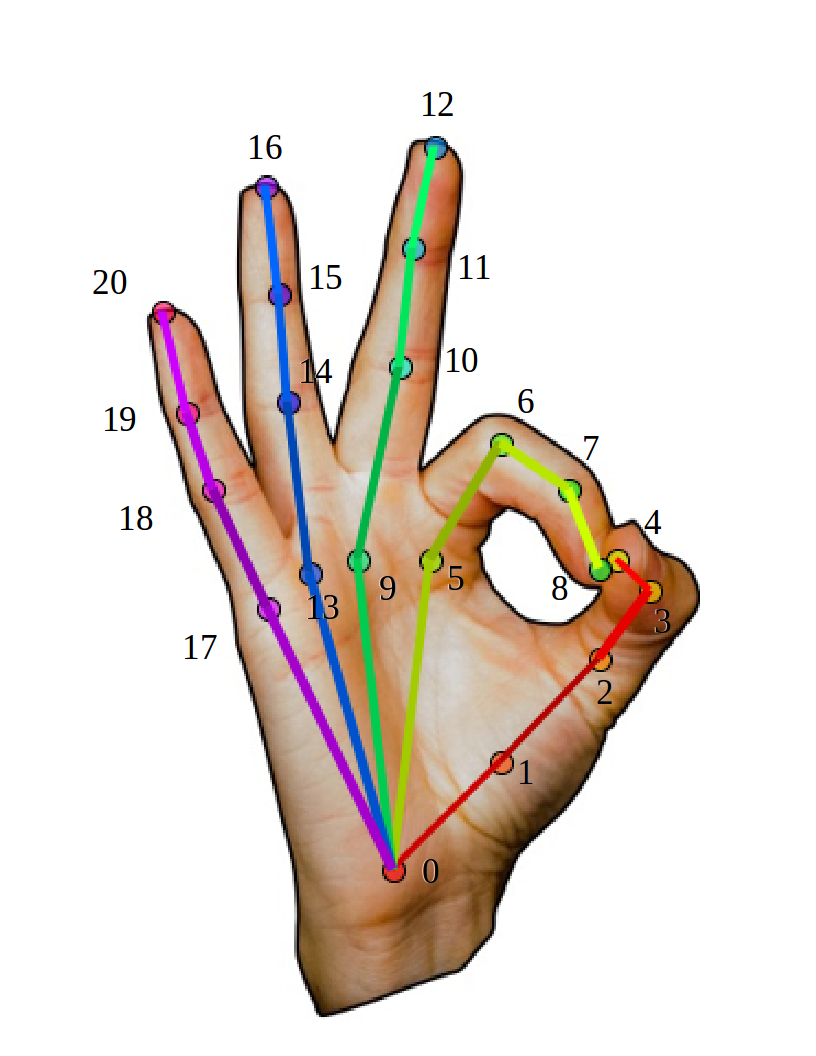
\includegraphics[width=2.5cm]{images/keypoints_hand}
    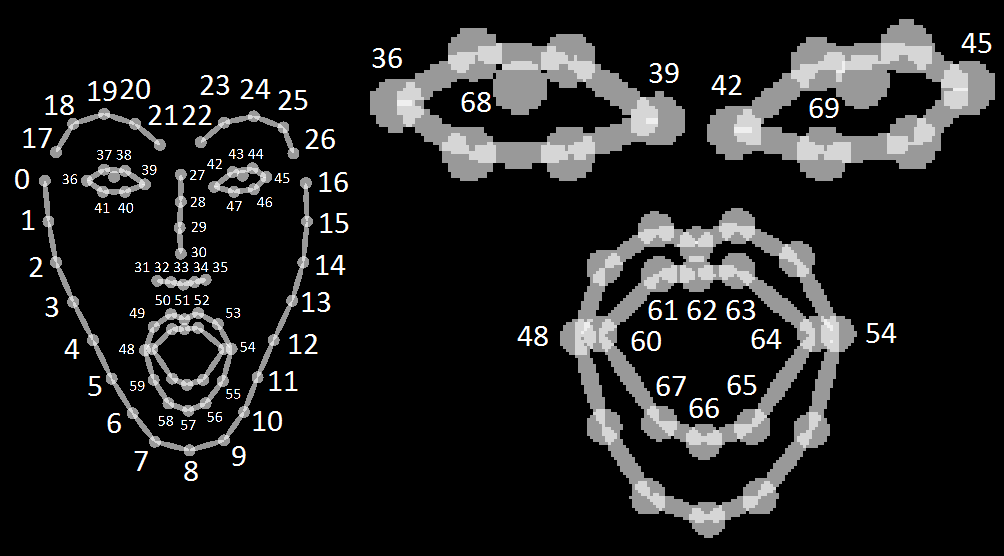
\includegraphics[width=4cm]{images/keypoints_face}
    \caption{Representação dos 21 pontos da mão (à esquerda) e 70 pontos da face (à direita), extraídos pelo OpenPose. Fonte: \cite{openpose-output-2018}.}
    \label{fig:keypoints-face-hand}
\end{figure}

\begin{figure}[ht]
    \centering
    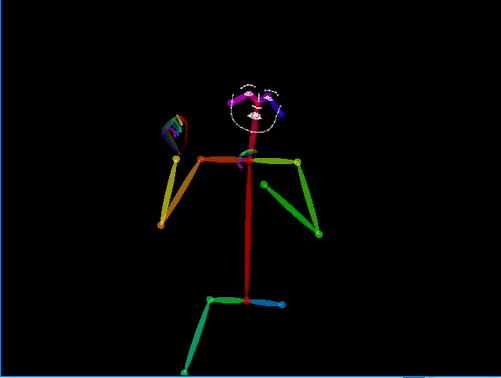
\includegraphics[width=3.5cm]{images/sign_pose}
    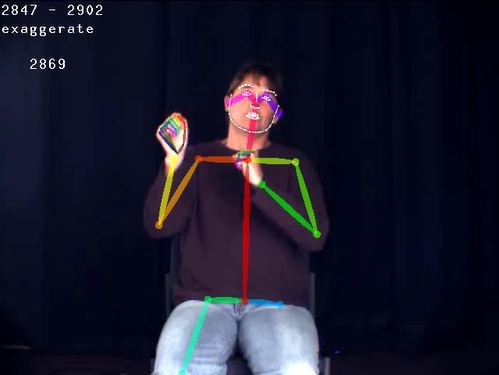
\includegraphics[width=3.5cm]{images/sign_pose_blended}
    \caption{Reconstrução do esqueleto a partir das coordenadas estimadas pelo OpenPose para um \textit{frame} do sinal "EXAGGERATE" (esquerda); e sobreposição desse esqueleto no vídeo original (direita). Fonte: OpenPose.}
    \label{fig:sign-pose}
\end{figure}

A figura \ref{fig:openpose-coordinates} mostra um exemplo de arquivo obtido ao final dessa etapa. Nele estão contidos para cada \textit{frame} uma seção denominada \textit{pose} com as coordenadas dos eixos X e Y estimadas para cada articulação do corpo, e uma seção \textit{score} que contempla o grau de confiança para a estimativa de cada uma dessas articulações..

\image
    [6cm]
    {fig:openpose-coordinates}
    {images/openpose_coordinates}
    {Exemplo de arquivo contendo as coordenadas estimadas para os esqueletos de cada sinal. Para cada \textit{frame} está contida uma seção \textit{pose} com as coordenadas X e Y estimadas para cada articulação, e uma seção \textit{score} com o grau de confiança da estimativa de cada uma dessas articulações.}

A quarta etapa diz respeito à \textbf{divisão do \textit{dataset}} processado até aqui em subconjuntos menores que serão utilizados para o treinamento e testes do modelo. Para esse procedimento, foi utilizada uma ferramenta de divisão de \textit{datasets} para validação cruzada denominada "\textit{train\_test\_split}", que é disponibilizada pela biblioteca Scikit-Learn \cite{scikit-learn}. Nessa divisão, foi considerada uma proporção de 80\% das amostras para treinamento (que corresponde a 7.798 itens) e 20\% para testes (correspondendo a 1.950 itens). Essa é uma proporção comumente adotada e entende-se que o número de amostras separadas para cada etapa é suficiente para validar o desempenho da grande parte dos modelos de aprendizagem de máquina.

Por fim, a quinta etapa consiste em \textbf{normalizar e serializar} as amostras afim de torná-las compatíveis com o formato de leitura do ST-GCN. A normalização objetiva tornar o comprimento de todas as amostras uniforme, aplicando para isso a repetição de seus \textit{frames} de forma sequencial até o preenchimento completo de um número fixo estabelecido de \textit{frames}. O número aqui adotado é de 63 \textit{frames} (que a uma taxa de 30 FPS, corresponde a um vídeo de duração aproximada de 2 segundos). A serialização, por sua vez, consiste em pré-carregar as amostras dos subconjuntos criados acima para traduzi-las em arquivos físicos do Python \cite{python}, contendo as respectivas representações em memória desses objetos. Esse é o formato de entrada esperado pelo ST-GCN, que é adotado para otimizar o processo de leitura dos dados. Para cada subconjunto acima são criados dois arquivos físicos: um contendo sua lista de amostras e outro contendo a lista de rótulos para essas amostras. 

O resultado do processamento de cada uma das etapas acima está disponibilizado individualmente no ASLLVD-Skeleton, conforme acima. O código fonte que realiza o processamento dessas etapas, por sua vez, está disponível juntamente com as adaptações do ST-GCN, conforme seção a seguir.


\subsection{Adaptação do ST-GCN para o reconhecimento de sinais} %%%%%%%%%%%%%%%%%%%%%%%%%%%%%%%%%%%%%%%%%%%%%%%%%%%%%%%%%%%%%%%%%%%%%%%%%%%
\label{sec:adaptacao-st-gcn}

Uma vez que a abordagem de representação por meio de grafos adotada pelo ST-GCN é bastante flexível, não foi necessário neste trabalho realizar modificações na arquitetura do modelo. Ao invés disso, apenas adaptações pontuais para fazer com que ele passasse a considerar as novas coordenadas para o domínio da língua de sinais foram realizadas. 

Dessa forma, foi criado um novo \textit{layout} de grafo para o problema atual, denominado "openpose-sl" contemplando as 130 articulações e suas relações. Além disso, foi necessário realizar ajustes nas dimensões de matrizes utilizadas no mecanismo de leitura dos dados para possibilitar com que eles comportassem as novas dimensões.

O código fonte contendo essas adaptações, bem como a implementação da sequência completa de etapas de pré-processamento está disponível publicamente\footnote{
    Disponível em \url{http://www.cin.ufpe.br/~cca5/st-gcn-sl}
}. Esse código consiste num \textit{fork} criado a partir daquele originalmente desenvolvido pelos autores em \cite{st-gcn-2018}.



\subsection{Experimentos} %%%%%%%%%%%%%%%%%%%%%%%%%%%%%%%%%%%%%%%%%%%%%%%%%%%%%%%%%%%%%%%%%%%%%%%%%%%
\label{experimentos}

Para este trabalho, foram utilizados como referência os experimentos apresentados em \cite{lim-2016}, o qual avalia a performance do reconhecimento dos sinais no \textit{dataset} ASLLVD pela técnica BHOF (vide seção \ref{sec:trabalhos-relacionados}) e também por técnicas populares como \textit{Motion Energy Image} (MEI) \cite{athitsos-asllvd-2008}, \textit{Motion History Image} (MHI) \cite{babu-2004}, \textit{Principal Component Analysis} (PCA) \cite{dreuw-2012} e \textit{Histogram of Optical Flow} (HOF) \cite{laptev-2008}. 

\begin{table}[]
\caption{Sinais selecionados para os experimentos em \cite{lim-2016}.}
\label{tab:asllvd-20}
\begin{tabular}{ll}
\hline
Dataset & Sinais selecionados \\ \hline
ASLLVD & \begin{tabular}[c]{@{}l@{}}adopt, again, all, awkward, baseball, behavior, can, chat, \\ cheap, cheat, church, coat, conflict, court, deposit, depressed, \\ doctor, don’t want, dress, enough\end{tabular} \\ \hline
\end{tabular}
\end{table}

Com esse propósito, os autores utilizaram um subconjunto contendo 20 sinais selecionados a partir do ASLLVD, conforme apresenta a tabela \ref{tab:asllvd-20}. Para reproduzir essa configuração, foram selecionadas as poses com esqueletos estimados para esse sinais a partir do \textit{dataset} criado na seção \ref{sec:criacao-dataset}. Como o número resultante de amostras é pequeno, totalizando 185 itens, foi necessário aplicar uma nova divisão fazendo com que 67\% desse subconjunto fosse separado para treinamento e 33\% para testes. Com isso, obteve-se um equilibrar maior no número de amostras uma avaliação mais adequada do modelo. Por fim, uma vez que tem-se uma nova divisão, foi necessário normalizar e serializar os novos suconjuntos para compatibilizá-los com o ST-GCN. Nesse processo adotou-se o mesmo procedimento apresentado na seção \ref{sec:criacao-dataset}. O subconjunto resultante, denominado de \textbf{ASLLVD-Skeleton-20} também foi disponibilizado publicamente\footnote{
    Disponível em \url{http://www.cin.ufpe.br/~cca5/asllvd-skeleton-20}
}.

Ainda devido às características desse conjunto de dados pequeno, o tamanho do \textit{batch} utilizado para o treinamento precisou ser reduzido para que melhores resultados passassem a ser observados nos experimentos. Dessa forma, após algumas tentativas frustradas com \textit{batches} maiores, passou-se a considerar um tamanho de 8 amostras.

Da mesma forma como na implementação original do algoritmo de treinamento do ST-GCN em \cite{st-gcn-2018}, os experimentos deste trabalho utilizaram como método de otimização o Gradiente Descendente Estocástico (ou \textit{Stochastic Gradient Descent} - SGD) com Momento de Nesterov, que por sua vez é capaz de melhorar a estabilidade e a convergência do SGD, como descrevem \cite{stanford-2018, bengio-2013, sutskever-2013}.

Para a taxa de aprendizagem, foi aplicada uma estratégia de inicializa-la com um valor elevado afim de que os pesos aleatórios sejam colocados na direção de convergência dentro das primeiras épocas. Em seguida, essa taxa foi reduzida gradativamente nas épocas posteriores possibilitando ajustes cada vez mais refinados dos pesos no treinamento. Dessa forma, no experimento com os 20 sinais selecionados foi utilizado um total de 600 épocas adotando uma taxa inicial de 0.1, a qual foi decaída para os valores de 0.01, 0.001, 0.0001 e 0.00001 após o término do treinamento das épocas 50, 250, 350 e 450, respectivamente.

% TODO: revisar configurações do experimento

Além do treinamento com o subconjunto de 20 sinais, também foi conduzido um experimento com o \textit{dataset} completo do ASLLVD, afim de estabelecer um valor de referência para ele. Para isso, apenas as configurações relacionadas ao tamanho do \textit{batch} e das épocas de decaimento da taxa de aprendizado precisaram ser alteradas. Sendo assim, o novo tamanho de \textit{batch} para esse cenário com muito mais amostras foi de 24 e a taxa de aprendizado teve comportamento de decaimento igual ao contexto acima, sendo aplicado ao término das épocas 100, 300, 400 e 500.

Os resultados obtidos em ambos os cenários estão apresentados na seção a seguir, e os modelos pré-treinados resultantes estão disponibilizados juntamente com as adaptações no ST-GCN, conforme seção seção \ref{sec:adaptacao-st-gcn}.


\section{Resultados} %%%%%%%%%%%%%%%%%%%%%%%%%%%%%%%%%%%%%%%%%%%
\label{sec:resultados}

Esta seção apresenta as descobertas e resultados obtidos a partir da aplicação da abordagem descrita nas seções anteriores. 

O primeiro experimento foi realizado utilizando a abordagem apresentada em \cite{lim-2016}, que considera a seleção de 20 sinais específicos do ASLLVD, e cujo desempenho está representado na figura \ref{fig:training-asllvd-20}. A linha vermelha apresenta a acurácia (\textit{top-1}) do modelo, e exibe sua evolução no decorrer das épocas de treinamento. Na linha cinza está representada a acurácia \textit{top-5}, que corresponde à acurácia com base nas 5 respostas de maior probabilidade apresentadas pelo modelo. Por fim, a linha tracejada azul representa evolução da taxa de aprendizagem utilizada nas respectivas épocas, e seu comportamento de decaimento.

\image
    [8.5cm]
    {fig:training-asllvd-20}
    {images/results_20}
    {Acurácia obtida pela abordagem apresentada no reconhecimento dos 20 sinais selecionados a partir do ASLLVD. A linha vermelha representa a acurácia Top 1 no decorrer das épocas de treinamento; a linha cinza, a acurácia Top 5; e a linha tracejada azul ilustra a taxa de aprendizagem utilizada e seu decaimento nas épocas respectivas.}

Pode-se perceber pela imagem que o modelo conseguiu alcançar de forma consistente uma acurácia de 35,85\% a partir da época 400 no reconhecimento dos sinais. A acurácia \textit{top-5}, por sua vez, foi capaz de alcançar um número de 64,15\%. Esse desempenho foi superior ao apresentado por técnicas tradicionais como o MEI e o MHI, mas não foi capaz de superar os resultados obtidos por técnicas como o PCA e o BHOF \cite{lim-2016}. A tabela \ref{tab:results-comparison-20} apresenta a comparação desses resultados com a abordagem proposta.

\begin{table}[ht]
\centering
\caption{Acurácia no reconhecimento de sinais utilizando diferentes abordagens, conforme proposto em \cite{lim-2016}.}
\label{tab:results-comparison-20}
\begin{tabular}{lc}
\hline
                   & Acurácia (\%)  \\ \hline
MHI                & 10.00                     \\
MEI                & 25.00                     \\
\textbf{ST-GCN SL} & \textbf{35.85}            \\
PCA                & 45.00                     \\
HOF                & 70.00                     \\
BHOF               & 85.00                     \\ \hline
\end{tabular}
\end{table}


% TODO: trocar imagem e revisar resultados do ASLLVD

Afim de estabelecer uma referência com o \textit{dataset} completo do ASLLVD, foi realizado um segundo experimento utilizado os seus 2.745 sinais. Nesse cenário, foi observada uma acurácia (\textit{top-1}) de 7,03\% e uma acurácia \textit{top-5} de aproximadamente 14,67\%. Certamente, trata-se de uma tarefa muito mais desafiadora do que a proposta em \cite{lim-2016} e os resultados obtidos refletem claramente essa complexidade. 

%\image
%    [8.5cm]
%    {fig:training-asllvd}
%    {images/results}
%    {Acurácia obtida no treinamento do \textit{dataset} completo ASLLVD. Na imagem estão ilustradas a acurácia Top 1, a acurácia Top 5 e a taxa de aprendizagem utilizada e seu decaimento no decorrer das épocas.}


Ao recapitular a abordagem proposta neste trabalho, percebe-se que uma de suas principais estratégias consiste em adotar um número maior de articulações afim de que partes do corpo não consideradas originalmente em \cite{st-gcn-2018}, como mãos e face, passassem a ser utilizadas para o reconhecimento da língua de sinais capturando diferentes aspectos de sua dinâmica. Isso fez com que o número de articulações aumentasse em mais de 7 vezes, partindo de 18 para 130. 

Contudo, os resultados obtidos nesses experimentos nos levam a acreditar que muitos desses 130 pontos não adicionaram informação significativa acerca do domínio do problema da língua de sinais para o modelo utilizado. Por exemplo, ao observar algumas amostras do ASLLVD apresentadas nas seções anteriores, perceberemos que os indivíduos estão sempre sentados e isso faz com que as coordenadas relacionadas a seus membros inferiores não sejam importantes; a face, por sua vez, contempla mais da metade das coordenadas utilizadas, porém muitos desses pontos não denotam movimentos expressivos para os sinais ou então são redundantes devido à grande densidade de coordenadas nessa região. 

Em contrapartida, o BHOF \cite{lim-2016} adota como objetivo centralizar o foco no movimento das mãos, isolando-as do restante do corpo e construindo histogramas a partir dos blocos nos \textit{frames} onde elas estão contidas durante a articulação dos sinais. De maneira efetiva, as mãos descrevem alguns dos principais traços nos movimentos da língua de sinais e, certamente o foco nelas e o sucesso em descartar informações pouco relevantes fizeram com que essa técnica apresentasse os resultados bastante expressivos com relação ao trabalho atual. Essa técnica é derivada do HOF e difere-se dele apenas pela abordagem de isolar as mãos dos indivíduos ao calcular o histograma do fluxo óptico.

Métodos como o MEI e MHI apresentam abordagens mais primitivas, que basicamente detectam os movimentos e sua intensidade a partir da diferença entre os \textit{frames} consecutivos das ações. Eles não são capazes de diferenciar indivíduos ou de focar em partes específicas de seu corpo, fazendo com que movimentos de qualquer natureza sejam considerados de maneira equivalente. O PCA, por sua vez, adiciona a capacidade de reduzir a dimensionalidade dos componentes utilizados com base na identificação daqueles de maior variância e que, consequentemente, são mais relevantes para a identificação do movimento nos \textit{frames}. 

Apesar dos resultados obtidos com a abordagem apresentados não terem alcançado um desempenho expressivo como o BHOF, que ele é capaz de apontar a direção para o desenvolvimento de novos estudos. Para trabalhos futuros, entende-se que há a necessidade de uma revisão no número de coordenadas utilizadas, eventualmente conduzindo uma avaliação do potencial de cada grupo delas em adicionar significância acerca do domínio do reconhecimento da língua de sinais.


% Bibliografia
\bibliographystyle{IEEEtran}
\bibliography{IEEEabrv,references.bib}

\end{document}
